\documentclass[12pt]{article}
\usepackage[utf8]{inputenc}
\usepackage[T1]{fontenc}
\usepackage{lmodern}  % for better quality fonts
\usepackage{amsmath,amssymb}
\usepackage{fontawesome}
\usepackage{lipsum}
\usepackage{hyperref}
\usepackage[margin=3em, top=0.5em]{geometry}
\usepackage{multirow}
\usepackage{array} % For extended tabular features
\usepackage{graphicx} % For better vertical alignment
\usepackage{xcolor}
\usepackage{titlesec}
\usepackage{tikz}
\usepackage{enumitem}


\definecolor{navy}{HTML}{1c398d}
\definecolor{softblack}{HTML}{333333}
\definecolor{subtextgray}{HTML}{768699}
\definecolor{LinkedinBlue}{HTML}{0a66c2}

\newcolumntype{L}[1]{>{\raggedright\arraybackslash}p{#1}}
\newcolumntype{R}[1]{>{\raggedleft\arraybackslash}p{#1}}

\setlength{\tabcolsep}{1.6em}

\renewcommand{\labelitemi}{\raisebox{0.1em}{$\cdot$}}

\begin{document}

\begin{center}
  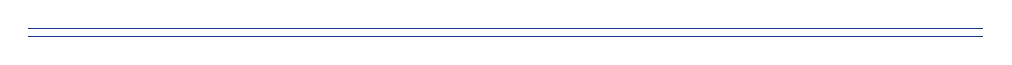
\begin{tikzpicture}
    \draw[thin, navy] (0,0) -- (\linewidth, 0);
    \draw[thin, navy] (0,-0.1) -- (\linewidth,-0.1);
  \end{tikzpicture}

  \vspace{0.4em}
  
  \begin{tabular}{@{} L{0.3\textwidth} c R{0.3\textwidth} @{}}
    \faEnvelope \hspace{0.1em} \color{softblack} \href{mailto:me@leosharif.com}{me@leosharif.com} & \color{softblack} \multirow{2}{*}{\huge\scshape Leo Sharif} & \faGithub \hspace{0.1em} \color{softblack} \href{https://github.com/Realaiz}{Leo Sharif} \\
    \faPhone \hspace{0.1em} \color{softblack} +61 420-677-719 & & \textcolor{LinkedinBlue} \faLinkedinSquare \hspace{0.1em} \color{softblack} \href{https://www.linkedin.com/in/leo-sharif-1a6866193/}{Leo Sharif} \\
    & \color{softblack} \normalsize \color{subtextgray} Mathematics \& Finance & \faHome \hspace{0.1em} \color{softblack} \href{https://leosharif.com}{leosharif.com} \\
  \end{tabular}

  \vspace{0.4em}

  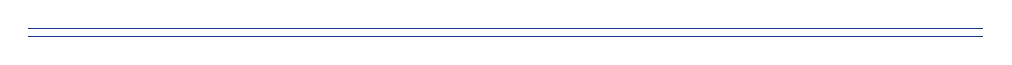
\begin{tikzpicture}
    \draw[thin, navy] (0,0) -- (\linewidth,0);
    \draw[thin, navy] (0,-0.1) -- (\linewidth,-0.1);
  \end{tikzpicture}
\end{center}


% Education Section
\section*{Education}
\textbf{Bond University} \hfill {Gold Coast, QLD}\\
\textit{\color{subtextgray}B. Actuarial Science, Major in Finance} \hfill \textit{\color{subtextgray}Feb 2022 - May 2024}
\begin{itemize}[noitemsep, topsep=0em, left=-0.8em]
  \item 75\% Major WAM, Investment Group, Actuarial Society, Tennis Club, Actuaries Institute of Australia Foundation Principles: CS1, CS2, CM1, CM2, CB1, CB2
  \item Coursework: Mathematical Statistics, Stochastic Processes, Econometrics, Financial Mathematics, Portfolio Analysis, Survival Analysis, Risk Management, Financial Models, Game Theory, Survival Analysis
\end{itemize}
\textbf{Academy of Interactive Technology} \\
\textit{\color{subtextgray}Diploma of Full Stack Development}
\begin{itemize}[topsep=0em, left=-0.8em]	
\item 78\% WAM, Developed a password manager and a real estate portfolio management tool, showcasing strong problem-solving skills and industry-standard security practices.
\end{itemize}

\end{document}



